\chapter[Toward a Stochastic Majority Vote]{Toward a Stochastic\\ Majority Vote}
\label{chap:mv-sto}

\addchapterlof
\addchapterloa
\addchapterloe

\vspace{-1.0cm}
\begin{center}
\textbf{This chapter is based on the following paper}\\[0.1cm]
\end{center}
\printpublication{ZantedeschiViallardMorvantEmonetHabrardGermainGuedj2021}

\vspace{0.2cm}
\minitoc

\begin{abstract}
We study a stochastic counterpart of the majority vote classifier called the {\it stochastic majority vote}, and study its generalization properties.
Unlike \Cref{chap:mv}, the posterior distribution associated with the majority vote is sampled from another probability distribution.
While the stochastic majority vote holds for arbitrary distributions, we instantiate it with Dirichlet distributions: this allows to derive a closed-form and differentiable expression for the expected risk.
Then, we derive self-bounding algorithms for stochastic majority vote, that benefit from tight generalization bounds when compared to self-bounding algorithms studied in \Cref{chap:mv}.
\end{abstract}

\newpage

\section{Introduction}

In \Cref{chap:mv}, we considered some self-bounding algorithms~\citep{Freund1998} that minimize a PAC-Bayesian bound on the majority vote true risk.
Each PAC-Bayesian bound depends on a surrogate on the majority vote risk (see \Cref{chap:pac-bayes:sec:surrogate}).
Given any distribution $\Q$ on an hypothesis set $\H$, we have seen three surrogates of the majority vote's risk in~\Cref{chap:pac-bayes}:
\begin{enumerate}[label={\it (\roman*)}]
    \item Twice the Gibbs Risk $r_{\dS}(\Q)=\EE_{(\x,\y)\sim\dS}   \EE_{\h\sim \Q} \indic\LB\h(\x) \ne \y\RB$ (\Cref{chap:pac-bayes:theorem:2gibbs}),
    \item 4 times the joint error $e_{\dS}(\Q)=\EE_{(\x,\y)\sim\dS} \EE_{\h\sim\Q}\EE_{\h'\sim\Q}
     \indic\LB\h(\x) \ne \y\RB\indic\LB\h'(\x) \ne \y\RB$ (\Cref{chap:pac-bayes:theorem:4joint}),
    \item The C-Bound $\CBound_{\dS}(\Q) = 1-\frac{\LP1-2r_{\dS}(\Q)\RP^2}{1-2d_{\dS}(\Q)}$, where $d_{\dS}(\Q)$ is the disagreement defined as $d_{\dS}(\Q)=2\EE_{(\x,\y)\sim\dS}\EE_{\h\sim\Q}\EE_{\h'\sim\Q}\indic\LB \h(\x)\ne \y\RB\indic\LB \h'(\x)=\y\RB$ (\Cref{chap:pac-bayes:theorem:cbound}).
\end{enumerate}

\Cref{chap:mv-sto:fig:moons-risk} illustrates the models obtained by the minimization of the empirical risk with respect to the three surrogates recalled above on a simple dataset (here, moons): only the empirical C-Bound fully leverage the diversity of the voters to obtain $\Risk_{\dS}(\MVQ)=0$.

\begin{figure}[H]
    \centering
    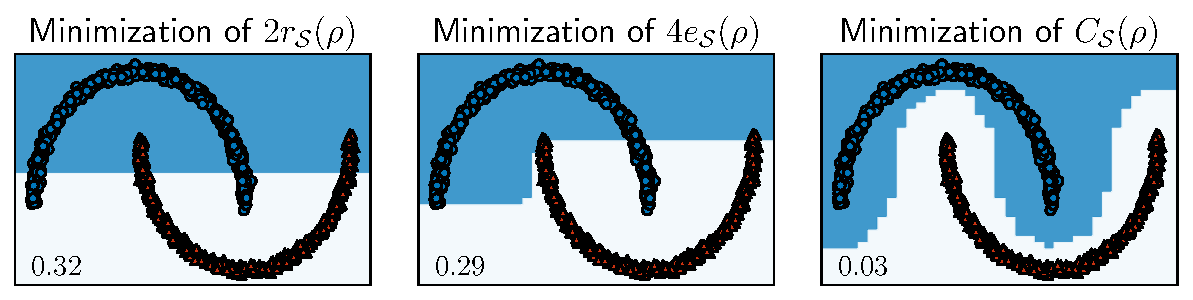
\includegraphics[width=1.0\linewidth]{chapter_5/figures/moons_risk.pdf}
    \caption[
    Comparison of the Minimization of the Surrogates on Moons]{Plot of the majority vote's decision boundary obtained by minimizing the upper bounds on the majority vote's empirical risk with the surrogates recalled in \Cref{chap:pac-bayes:theorem:2gibbs,chap:pac-bayes:theorem:4joint,chap:pac-bayes:theorem:cbound} for moons dataset with a learning sample size $\m=1,000$.
    For each plot, we print the surrogate value in the bottom left corner.
    }
    \label{chap:mv-sto:fig:moons-risk}
\end{figure}

\looseness=-1
As highlighted in \Cref{chap:mv-sto:fig:moons-risk}, the first two surrogates (\Cref{chap:pac-bayes:theorem:2gibbs,chap:pac-bayes:theorem:4joint}) are not efficient to minimize the empirical majority vote's risk.
In contrast, since the empirical C-Bound $\CBound_{\dS}(\Q)$ (\Cref{chap:pac-bayes:theorem:cbound}) is a tighter upper bound on the majority vote's empirical risk (\Cref{chap:pac-bayes:theorem:relationship}), the minimization of the empirical risk through the C-Bound is more accurate.
Another precise surrogate on the majority vote's empirical risk is based on the {\it randomized majority vote}.
This model, introduced by \citet{LacasseLavioletteMarchandTurgeonBoutin2010}, consists in defining a majority vote
\begin{align*}
    \MVQrand(\x) \defeq \argmax_{\y'\in\Y}\EE_{\h\sim\Qrand}\indic\LB \h(\x) = \y'\RB,
\end{align*}
where $\Qrand$ is constructed as follows: $N$ voters $\Hp=\{\h_1,\dots,\h_N\}$ are sampled from $\Q$ and a uniform posterior distribution $\Qrand$ is defined such that $\Qrand(\h)=\frac{1}{N}$ for all $\h\in\Hp$.
Following~\citet{LacasseLavioletteMarchandTurgeonBoutin2010}, the randomized majority vote's empirical risk is defined as
\begin{align*}
&\hspace{-1cm}\PP_{(\x,\y)\sim\dS, \MVQrand\sim\Q^N}\LB\MVQrand(\x)\ne \y\RB\\ &\le \EE_{(\x,\y)\sim\S}\LB\sum_{j=\lceil\frac{N}{2}\rceil}^N\binom{N}{j} \LB\frac{1}{2}\LP1-\OmMaQ(\x,\y)\RP\RB^j \LB1-\frac{1}{2}\LP1-\OmMaQ(\x,\y)\RP\RB^{(N-j)}\RB\\
&\defeq b_{\S}^{N}(\Q),\\
\end{align*}
where $\OmMaQ(\x,\y)$ is the $\frac{1}{2}$-margin defined in \Cref{chap:pac-bayes:def:1/2-margin}.
Given an example $(\x,\y)\sim\S$, the sum corresponds to the probability that at least $\frac{N}{2}$ voters make an error over $N$ voters sampled from $\Q$.
In fact, it is the complementary cumulative distribution function of the binomial distribution with parameter $\tfrac{1}{2}(1-\OmMaQ(\x,\y))$ and $\lceil\frac{N}{2}\rceil$ trials.
Hence, $b_{\S}^{N}(\Q)$ is the expected complementary cumulative distribution function on the learning sample $\S$.
Moreover, the {\it randomized} majority vote can be linked to the classical majority vote $\MVQ$: the term $b_{\dS}^{N}(\Q)$ is another surrogate on the majority vote empirical risks~\citep{LacasseLavioletteMarchandTurgeonBoutin2010}.
Indeed, we have
\begin{align}
    \Risk_{\dS}(\MVQ) \le 2b_{\dS}^{N}(\Q).\label{chap:mv-sto:eq:lacasse}
\end{align}
Note that we provide a proof of this bound in \Cref{ap:mv-sto:sec:algolacasse}.
Hopefully, the higher $N$, the better $b_{\dS}^{N}(\Q)$ approximates the majority vote's empirical risk risk.
As for the other surrogates (\ie, the Gibbs risk, the joint error, and the C-Bound), when one wants to upper-bound the majority vote's true risk, PAC-Bayesian bounds are used.
In the rest of the chapter, we denote by \algolacasse our algorithm that minimizes a PAC-Bayesian bound depending on $b_{\dS}^{N}(\Q)$ (see \Cref{ap:mv-sto:sec:algolacasse}).
However, when the true risk is minimized through self-bounding algorithms, it gives even worse results on the moons dataset.
This is illustrated on \Cref{chap:mv-sto:fig:moons-bound} that plots the different self-bounding procedures.

\begin{figure}
    \centering
    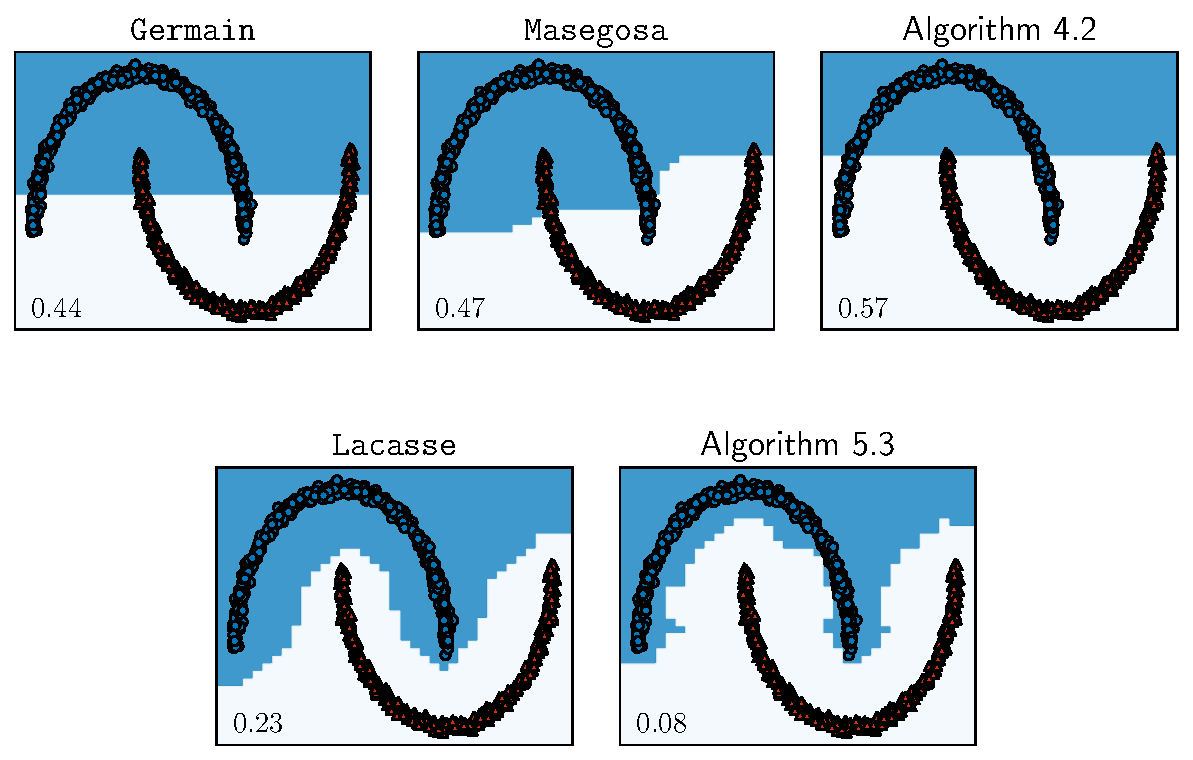
\includegraphics[width=1.0\linewidth]{chapter_5/figures/moons_bound.pdf}
    \caption[Comparison of the Self-bounding Algorithms on Moons]{Plot of the majority vote's decision boundary obtained by executing the self-bounding algorithms for moons dataset with $\m=1,000$ (and $N = 100$ for \algolacasse).
    We represent in the bottom left of the plots, the value of each bound minimized with \Cref{chap:mv:algo:seeger}, \Cref{chap:mv-sto:algo:not-data} (and \Cref{chap:mv-sto:algo:exact}), \algogermain~(\Cref{ap:mv:algo:2-gibbs}), \algomasegosa~\citep[Appendix~G]{MasegosaLorenzenIgelSeldin2020}, and \algolacasse~(\Cref{chap:mv-sto:algo:lacasse}). 
    }
    \label{chap:mv-sto:fig:moons-bound}
\end{figure}

As we can remark, except for the one labelled \algolacasse and our new \Cref{chap:mv-sto:algo:not-data}, the minimization of the PAC-Bayesian bounds does not fully leverage the voters' correlations to obtain a {\it (i)} tight generalization bound and {\it (ii)} a small empirical risk.
This is mainly due to the fact that they do not minimize directly the majority vote's risk (but surrogates instead).
In contrast, as illustrated by \citet{Lacasse2010}'s result, the randomized majority vote offers a way to obtain a tight generalization guarantee with a small empirical risk $\Risk_{\dS}(\MVQ)$.
However, the considered majority vote in \citet{LacasseLavioletteMarchandTurgeonBoutin2010}'s approach is not the original majority vote $\MVQ$, but a rather restricted form.

Hence, in this chapter, we introduce the {\it stochastic} majority vote that overcomes the drawbacks of the literature's methods: we provide tight generalization bounds on the classical majority vote $\MVQ$.
The {\it stochastic} majority vote is defined as follows: for each input $\x$, a majority vote $\MVQ$ is obtained by sampling the weights from another probability distribution.

This new majority vote is presented in more details in \Cref{chap:mv-sto:sec:mv-sto}; its definition is given in \Cref{chap:mv-sto:sec:def}.
Moreover, we show in \Cref{chap:mv-sto:sec:mc} how to approximate the risk and in \Cref{chap:mv-sto:sec:exact} the exact computation.
Along with the risk computation, we derive in \Cref{chap:mv-sto:sec:bound,chap:mv-sto:sec:bound-data} two PAC-Bayesian bounds essential to derive self-bounding algorithms in \Cref{chap:mv-sto:sec:algo}.
\Cref{chap:mv-sto:sec:expe} provides a study of these algorithms.
The proofs are deferred in \Cref{ap:mv-sto}. 

\section{The Stochastic Majority Vote}
\label{chap:mv-sto:sec:mv-sto}


\subsection{Definitions}
\label{chap:mv-sto:sec:def}

For the {\it stochastic} majority vote, we consider that its weights $\Q\in\M(\H)$ are sampled from a distribution $\hyperQ$ called hyper-posterior\footnote{The hyper-posteriors have been first used in the PAC-Bayesian theory by \citet{PentinaLampert2014} in the context of Life-long learning problem in order to be able to consider different majority votes adapted to the different specific tasks seen during training.}; we say that $\hyperQ$ is a hyper-posterior on $\H$.
By considering hyper-posteriors, the majority votes become {\it stochastic}, \ie, for each input $\x\in\X$ the weights $\Q$ are sampled from the hyper-posterior $\hyperQ$ to obtain the prediction $\MVQ(\x)$.
The main advantage of considering a stochastic majority vote is that it allows to derive and to optimize PAC-Bayesian generalization bounds directly.
The true risk and empirical risk of the proposed stochastic weighted majority vote take into account the risks of $\MVQ$ where $\Q$ is sampled from the hyper-posterior $\hyperQ$; the risk is defined in the following definition.

\begin{definition}[Risks of the stochastic majority vote] For any distribution $\D$ on $\X{\times}\Y$, for any  for any voters' set $\H$, for any hyper-posterior distribution $\hyperQ$ on $\H$, the stochastic risks are defined as
\begin{align*}
    &\EE_{\Q\sim\hyperQ}\Risk_{\D}(\MVQ) = \EE_{\Q\sim\hyperQ}\EE_{(\x,\y)\sim\D}
    \indic\LB \MaQ(\x, \y) \le 0\RB,\\
    \text{and}\quad &\EE_{\Q\sim\hyperQ}\Risk_{\dS}(\MVQ) = \EE_{\Q\sim\hyperQ}\frac{1}{\m}\sum_{i=1}^{\m}
    \indic\LB \MaQ(\x_i, \y_i) \le 0\RB.
\end{align*}
\end{definition}

We use the $\frac{1}{2}$-margin of \citet{LavioletteMorvantRalaivolaRoy2017} to upper-bound the risk of the stochastic majority vote.
Indeed, we have
\begin{align}
    &\EE_{\Q\sim\hyperQ}\Risk_{\D}(\MVQ) \le \EE_{\Q\sim\hyperQ}\EE_{(\x,\y)\sim\D}
    \indic\LB \OmMaQ(\x, \y) \le 0\RB = \EE_{(\x,\y)\sim\D}s_{\hyperQ}(\x,\y),\label{chap:mv-sto:eq:true-sto-risk}\\
    \text{and}\quad &\EE_{\Q\sim\hyperQ}\Risk_{\dS}(\MVQ) \le \EE_{\Q\sim\hyperQ}\frac{1}{\m}\sum_{i=1}^{\m}
    \indic\LB \OmMaQ(\x_i, \y_i) \le 0\RB = \frac{1}{\m}\sum_{i=1}^{\m}s_{\hyperQ}(\x_i,\y_i).\label{chap:mv-sto:eq:emp-sto-risk}
\end{align}
where $s_{\hyperQ}(\x,\y) \triangleq \EE_{\Q\sim\hyperQ}\indic\LB \OmMaQ(\x, \y) \le 0\RB$ is the {\it stochastic} risk.
Note first that the inequality is attained in the binary setting (see \Cref{chap:pac-bayes:sec:surrogate}).
Additionally, the advantage of $s_{\hyperQ}(\x,\y)$ is that we are able to derive a closed form solution in \Cref{chap:mv-sto:sec:exact}.
Actually, we introduce two ways to compute this risk: we can either {\it (i)} approximate it (\eg, through Monte Carlo methods) or {\it (ii)} compute its closed form.
In both cases, assumptions have to be made on the distribution $\hyperQ$.
When the distribution $\Q$ is discrete, it lies in the ($\card(\H){-}1$) dimensional probability simplex: $\deltabb^{(\card(\H){-}1)}$.
Hence, a natural choice for the hyper-posterior is the Dirichlet  distribution; its probability density function is defined as follows.
\begin{definition}[Dirichlet Distribution] Let $\n=\card(\H)$ be the cardinality of a finite hypothesis set $\H$. 
Given the concentration parameters $\paramDir\in(\Rbb^{+}_{*})^\n$, the Dirichlet Distribution $\Dir(\paramDir)$ is defined as
\begin{align*}
    \Q\sim\hyperQ \iff (\Q(\h_1),\dots,\Q(\h_\n)) \sim\Dir(\paramDir),\\
    \text{where}\quad \hyperQ(\Q) \triangleq \frac{1}{Z(\paramDir)}\prod_{j=1}^\n \Big[\Q(\h_j)\Big]^{\sparamDir_j-1} \propto \prod_{j=1}^\n \Big[\Q(\h_j)\Big]^{\sparamDir_j-1}.
\end{align*}
\label{chap:mv-sto:def:dirichlet}
\end{definition}

We provide in \Cref{chap:mv-sto:fig:dirichlet} some examples of Dirichlet distributions.
Notice that by taking $\paramDir$ as the vector of all ones, the distribution corresponds to a uniform distribution over the simplex $\deltabb^{(\card(\H){-}1)}$.

\begin{figure}
\centering
\begin{subfigure}{0.32\textwidth}
    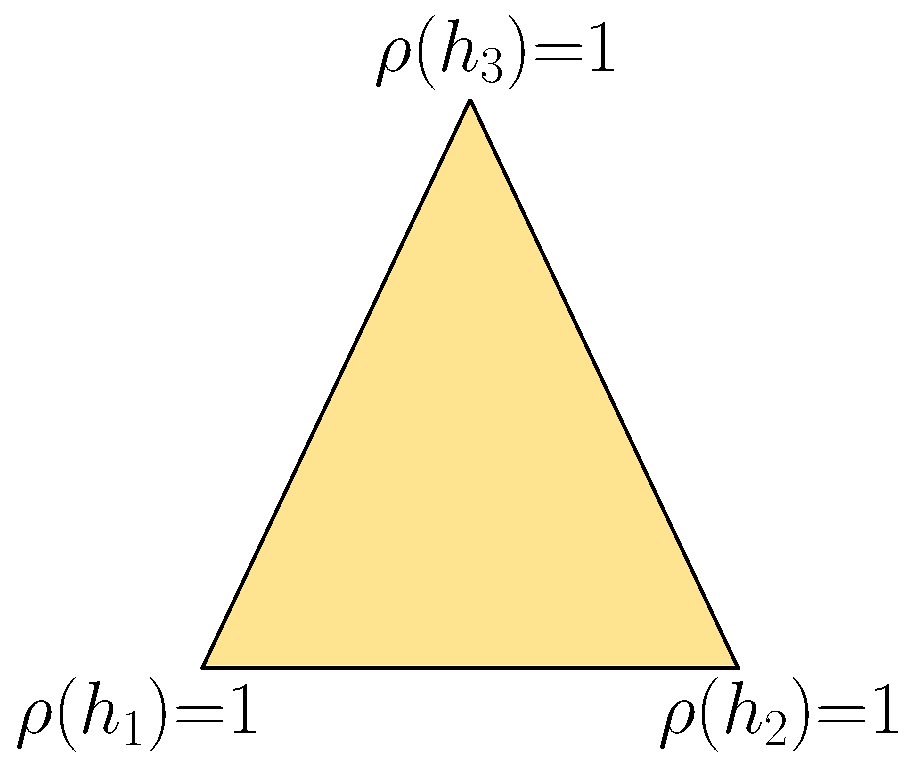
\includegraphics[width=\textwidth]{chapter_5/figures/dirichlet_1_1_1.pdf}
    \caption{$\paramDir=[1, 1, 1]^{\top}$}
\end{subfigure}
\hfill
\begin{subfigure}{0.32\textwidth}
    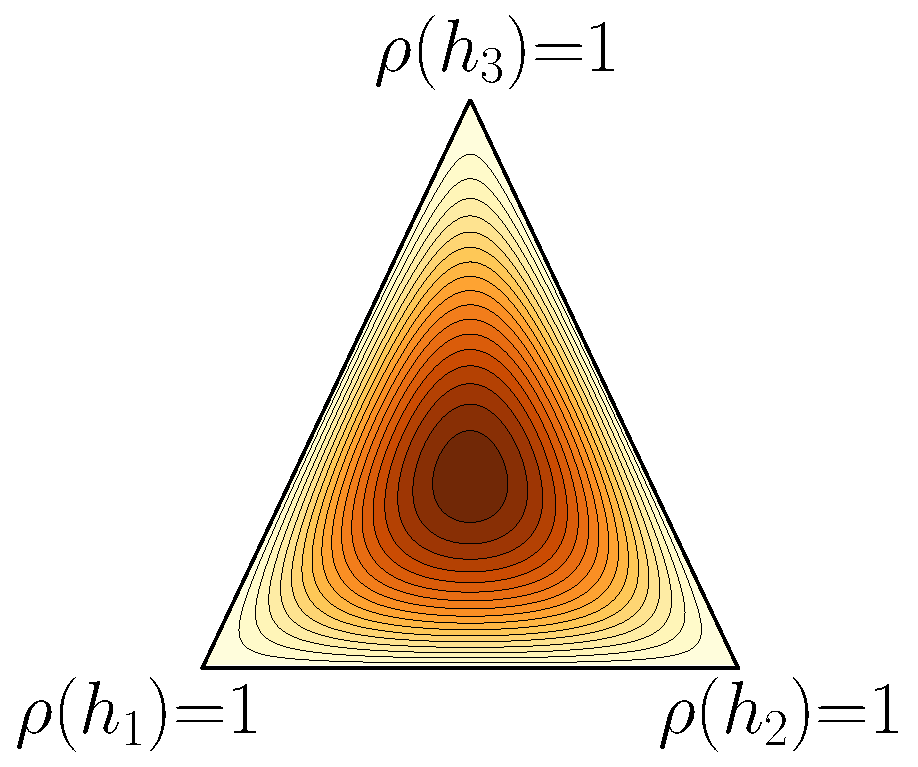
\includegraphics[width=\textwidth]{chapter_5/figures/dirichlet_2_2_2.pdf}
    \caption{$\paramDir=[2, 2, 2]^{\top}$}
\end{subfigure}
\hfill
\begin{subfigure}{0.32\textwidth}
    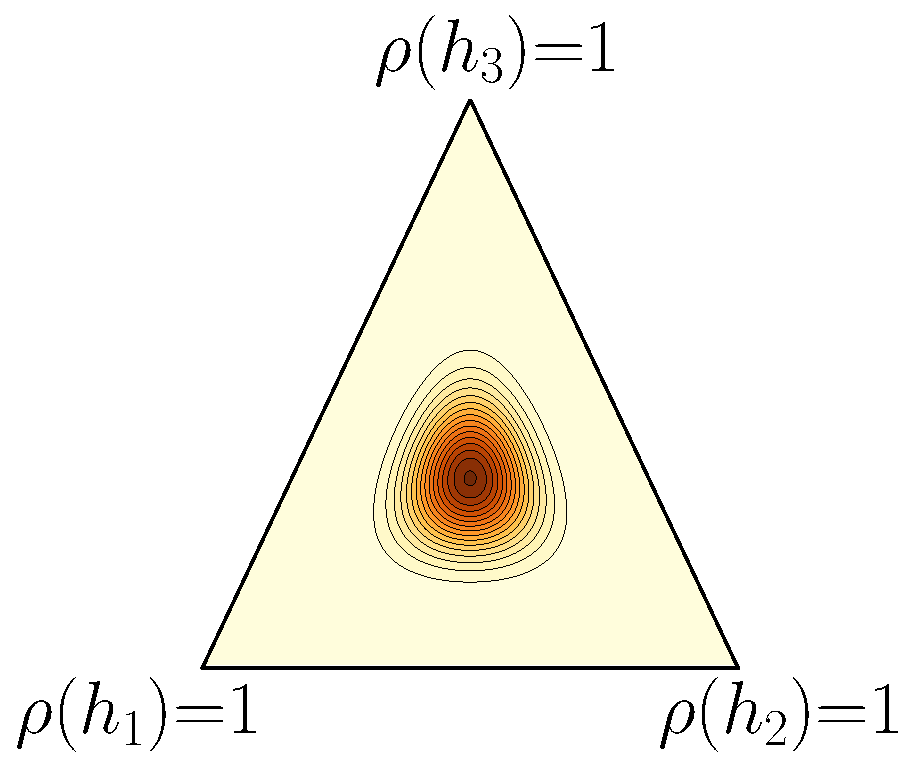
\includegraphics[width=\textwidth]{chapter_5/figures/dirichlet_10_10_10.pdf}
    \caption{$\paramDir=[10, 10, 10]^{\top}$}
\end{subfigure}

\begin{subfigure}{0.32\textwidth}
    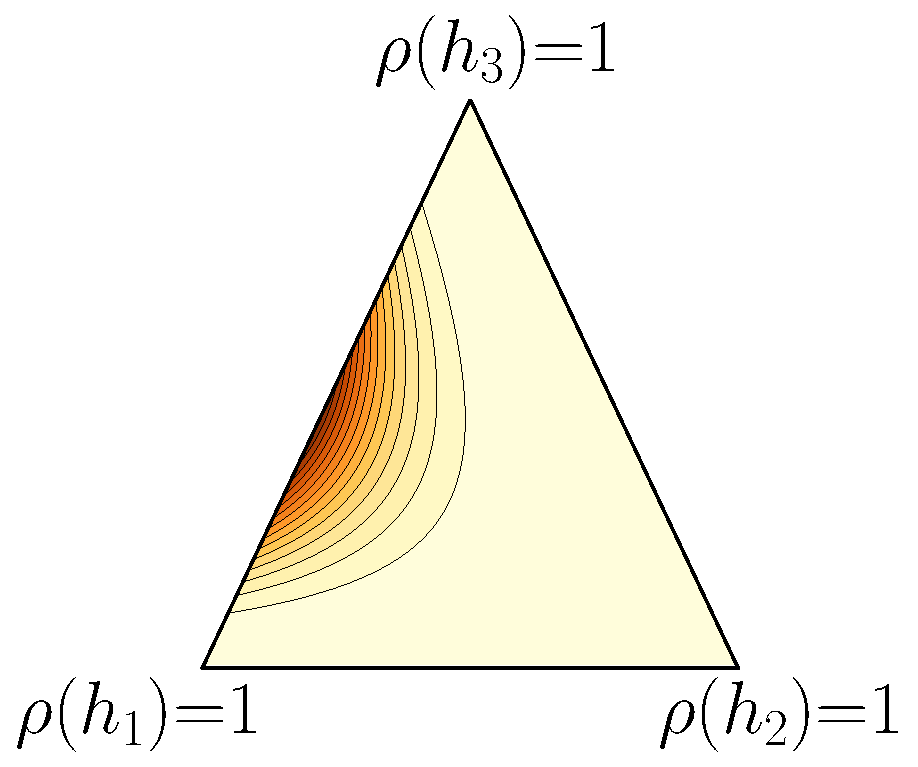
\includegraphics[width=\textwidth]{chapter_5/figures/dirichlet_5_1_4.pdf}
    \caption{$\paramDir=[5, 1, 4]^{\top}$}
\end{subfigure}
\hfill
\begin{subfigure}{0.32\textwidth}
    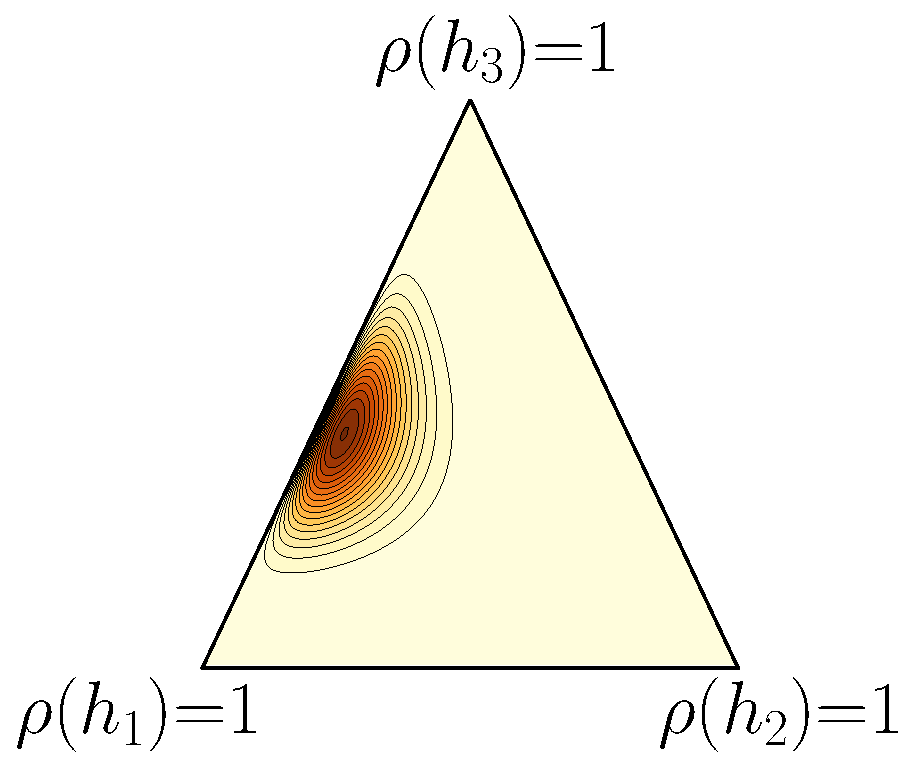
\includegraphics[width=\textwidth]{chapter_5/figures/dirichlet_10_2_8.pdf}
    \caption{$\paramDir=[10, 2, 8]^{\top}$}
\end{subfigure}
\hfill
\begin{subfigure}{0.32\textwidth}
    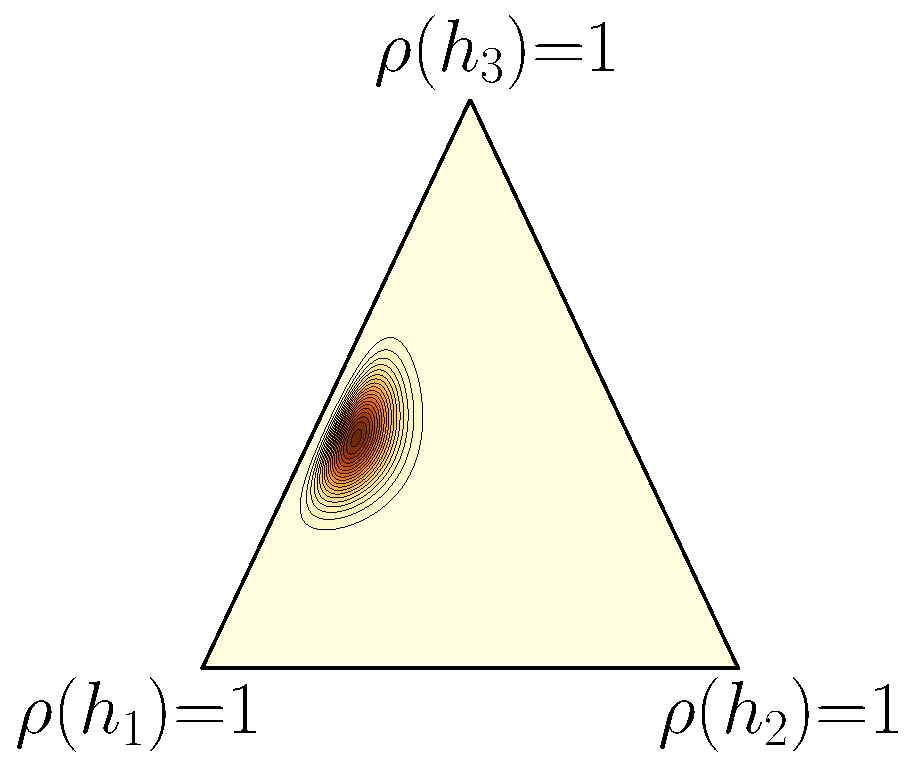
\includegraphics[width=\textwidth]{chapter_5/figures/dirichlet_25_5_20.pdf}
    \caption{$\paramDir=[25, 5, 20]^{\top}$}
\end{subfigure}
        
\caption[Examples of Probability Density Functions for the Dirichlet Distribution]{The figure shows the probability density function for different value of parameters $\paramDir$. 
More precisely, the ``triangle'' correspond to the $2$-dimensional probability simplex $\simplex^2$ where its extremities correspond to the extreme probability distributions. 
Hence, a point in the simplex is a linear combination of these extreme probability distributions.
}
\label{chap:mv-sto:fig:dirichlet}
\end{figure}


Under Dirichlet assumptions on the hyper-posterior distribution $\hyperQ$, we propose in the next section an algorithm to approximate the stochastic risk $s_{\hyperQ}(\x,\y)$.
This algorithm is actually part of our self-bounding algorithm in \Cref{chap:mv-sto:sec:algo}.

\subsection{Approximation of the Stochastic Risk}
\label{chap:mv-sto:sec:mc}

We now propose a Monte Carlo (MC) algorithm to compute $s_{\hyperQ}(\x,\y)$ that is suited to speed up the optimization.
For this optimization algorithm, we need to introduce a surrogate of the true risk to update $\paramDir$ by gradient descent as the gradients of the $01$-loss are always zero.
We make use of a \emph{tempered} sigmoid loss $\sig_c(x) = \frac{1}{1+\exp(-cx)}$ with slope parameter $c \in \R^{+}$.
Because of the surrogate, this optimization algorithm solves a relaxation of the original problem and not its exact form~\citep{Nesterov2005}.
The MC-based optimization algorithm is described in \Cref{chap:mv-sto:algo:mc}.

\begin{algorithm}[H]
 \caption{Approximating the Stochastic Risk}
  \begin{algorithmic}
  \State{{\bf Given: } Dirichlet distribution $\hyperQ=\Dir(\paramDir)$, learning sample $\S$}
  \State{{\bf Hyperparameters: } number of draws $\K$}
  \State{Draw a sample $\{\Q_\k\}_{\k=1}^\K \sim \hyperQ^\K=\Dir(\paramDir)^\K$}
  \For{{\bf all} example $(\x_i,\y_i)\in\S$}
    \State{\centerline{$\displaystyle s_{\hyperQ}(\x_i,\y_i) \approx \frac{1}{\K}\sum_{\k=1}^\K \sig_c\LB -\OmMaQk(\x_i,\y_i) \RB$}}
  \EndFor
  \Return{$\frac{1}{\m}\sum_{i=1}^{\m}s_{\hyperQ}(\x_i,\y_i)$}
  \end{algorithmic}
  \label{chap:mv-sto:algo:mc}
\end{algorithm}

This algorithm first samples $\K$ majority votes and computes an approximation of the stochastic risk $s_{\hyperQ}(\x_i,\y_i)$ for each example $(\x_i,\y_i)\in\S$ by an average.
A drawback of \Cref{chap:mv-sto:algo:mc} is that it requires to sample $\K$ majority votes and predict all the examples in the learning sample $\S$.
Hence, to overcome this issue, we derive a closed-form solution of the stochastic risk $s_{\hyperQ}(\x,\y)$ in the next section. 

\subsection{Computing Exactly the Stochastic Risk}
\label{chap:mv-sto:sec:exact}

Under Dirichlet assumptions, a closed-form solution can be derived for the expected risk.
The following lemma introduces this solution.

\begin{restatable}[Computation of the Stochastic Risk]{lemma}{lemmarisk}\label{chap:mv-sto:lemma:risk}
For a given $(\x, \y) \in \X{\times}\Y$, let 
\begin{align*}
\Fbb(\x, \y) = \LC j \;:\; \h_j(\x) \neq \y \RC \quad\text{and}\quad  \Tbb(\x, \y) = \LC j \;:\; \h_j(\x) = \y \RC
\end{align*}
\looseness=-1
 be respectively the set of indices of the voters that misclassify $(\x, \y)$ and the set of indices of the voters that correctly classify $(\x, \y)$. 
Then, the stochastic risk $s_{\hyperQ}(\x, \y)$ can be rewritten as
\begin{align*}
    s_{\hyperQ}(\x, \y) = \EE_{\Q\sim\hyperQ} \indic\LB \OmMaQ(\x, \y) \le 0\RB =  I_{0.5}\LP\sum_{j\in \Tbb(\x, \y)} \sparamDir_j, \sum_{j\in \Fbb(\x, \y)} \sparamDir_j\RP ,
\end{align*}
with $I_{0.5}()$ the regularized incomplete beta function evaluated at $0.5$.
It is defined as
\begin{align*}
I_{0.5}(a, b)\defeq \frac{B_{0.5}(a, b)}{B_1(a, b)}, \quad\text{where}\quad B_{t}(a, b) \defeq \int_{0}^{t}x^{a-1}(1-x)^{b-1}dx
\end{align*}
is the incomplete beta function.
\end{restatable}
\begin{noaddcontents}\begin{proof}
Deferred to~\Cref{chap:mv-sto:sec:proof-lemma-risk}.
\end{proof}\end{noaddcontents}

\Cref{chap:mv-sto:lemma:risk} tells us that the stochastic risk given an example $(\x, \y)$ can be computed with a closed-form solution.
In consequence, thanks to \Cref{chap:mv-sto:lemma:risk}, we compute an upper-bound on the risk of the stochastic majority vote based on the stochastic risk.
Indeed, we deduce the following corollary.

\begin{restatable}[Closed-form Solution of the Stochastic Risks]{corollary}{corollaryrisk}\label{chap:mv-sto:corollary:risk}
For any distribution $\D$ on $\X{\times}\Y$, for any learning sample $\S\sim\D^m$, for any finite hypothesis set $\H$, for any distribution $\hyperQ=\Dir(\paramDir)$ with $\paramDir\in(\Rbb^{+}_{*})^{\card(\H)}$, we have
\begin{align*}
&\EE_{\Q\sim\hyperQ}\Risk_{\D}(\MVQ) \le \EE_{(\x,\y)\sim\D}s_{\hyperQ}(\x, \y) = \EE_{(\x,\y)\sim\D} I_{0.5}\LP\sum_{j \in \Tbb(\x,\y)} \sparamDir_j, \sum_{j \in \Fbb(\x,\y)} \sparamDir_j\RP,\\
\text{and}\quad &\EE_{\Q\sim\hyperQ}\Risk_{\dS}(\MVQ) \le \frac{1}{\m}\sum_{i=1}^\m s_{\hyperQ}(\x_i, \y_i) = \frac{1}{\m}\sum_{i=1}^\m I_{0.5}\LP\sum_{j \in \Tbb(\x_i,\y_i)} \sparamDir_j, \sum_{j \in \Fbb(\x_i,\y_i)} \sparamDir_j\RP.
\end{align*}
\end{restatable}
\begin{noaddcontents}\begin{proof}
Deferred to~\Cref{chap:mv-sto:sec:proof-corollary-risk}.
\end{proof}\end{noaddcontents}

From \Cref{chap:mv-sto:corollary:risk}, we propose to compute directly the empirical stochastic risk.
This is in contrast with \Cref{chap:mv-sto:algo:mc} that approximates the stochastic risk by Monte Carlo sampling.
The computation is summarized in \Cref{chap:mv-sto:algo:exact}.
Note that we provide in~\ref{chap:mv-sto:sec:exact-mc} an empirical study showing in which regimes each algorithm is more efficient.

\begin{algorithm}[H]
 \caption{Computing Exactly the Stochastic Majority Vote's Risk}
  \begin{algorithmic}
  \State{{\bf Given: } Dirichlet distribution $\hyperQ=\Dir(\paramDir)$, learning sample $\S$}
    \For{{\bf all} example $(\x_i,\y_i)\in\S$}
        \State{
        \centerline{$\displaystyle s_{\hyperQ}(\x_i, \y_i) =  I_{0.5}\LP\sum_{j\in \Tbb(\x_i, \y_i)} \sparamDir_j, \sum_{j\in \Fbb(\x_i, \y_i)} \sparamDir_j\RP$}
        }
    \EndFor
  \Return{$\frac{1}{\m}\sum_{i=1}^{\m}s_{\hyperQ}(\x_i,\y_i)$}
  \end{algorithmic}
  \label{chap:mv-sto:algo:exact}
\end{algorithm}

Thanks to \Cref{chap:mv-sto:algo:mc} and \Cref{chap:mv-sto:algo:exact}, we are now able to compute the compute the empirical stochastic risk. 
This is a key step to derive our self-bounding algorithm in \Cref{chap:mv-sto:sec:algo} for the stochastic majority vote.
Indeed, the PAC-Bayesian generalization bound that we derive in the next section requires the computation of the stochastic risk in order to be minimized.

\section{From a PAC-Bayesian Bound to an Algorithm}

We now derive PAC-Bayesian generalization bounds for our proposed stochastic majority vote.
To do so, we upper-bound the true stochastic risk with a \citeauthor{Seeger2002}-like PAC-Bayesian bound.
More precisely, we propose in \Cref{chap:mv-sto:sec:bound} a PAC-Bayesian bound for a stochastic majority vote with voters that do not depend on the learning sample $\S$ and in \Cref{chap:mv-sto:sec:bound-data} we derive a PAC-Bayesian for data-dependent voters.

\subsection{A PAC-Bayesian Bound for Stochastic Majority Votes}
\label{chap:mv-sto:sec:bound}

Before presenting our PAC-Bayesian bound for the stochastic majority vote, we consider that we have an \apriori on the majority vote weights $\Q\in\M(\H)$, \ie, we assume a hyper-prior distribution $\hyperP$ over the voters' set $\H$.
By doing so, we are able to derive a bound that depends on the KL divergence $\KL(\hyperQ\|\hyperP)$ between the hyper-prior $\hyperP$ and the hyper-posterior $\hyperQ$.
Our bound is presented in the following theorem.

\begin{restatable}[PAC-Bayesian Bound for Stochastic Majority Votes]{theorem}{theorembound}\label{chap:mv-sto:theorem:bound}
For any distribution $\D$ on $\X{\times}\Y$, for any finite hypothesis set $\H$, for any distribution $\hyperP=\Dir(\paramDirP)$ with $\paramDirP\in(\Rbb^{+}_{*})^{\card(\H)}$, for any $\delta \in (0, 1]$, with probability at least $1-\delta$ over the random choice of $\S\sim\D^\m$, we have for all hyper-posterior $\hyperQ$ on $\H$ 
\begin{align*}
    &\hspace{-3.2cm}\EE_{\Q\sim\hyperQ}\Risk_{\D}(\MVQ) \le \EE_{(\x,\y)\sim\D}s_{\hyperQ}(\x, \y) \le \klmax\LP \frac{1}{\m}\sum_{i=1}^\m s_{\hyperQ}(\x_i, \y_i) \;\middle|\; \frac{\KL(\hyperQ\|\hyperP){+}\ln\frac{2\sqrt{m}}{\delta}}{\m}\RP,\\[0.5cm]
    \text{with}\quad \KL(\hyperQ\|\hyperP)&=\!\!\!\sum_{j=1}^{\card(\H)}\!\!\ln\!\LB\Gamma\LP\sparamDirP_j\RP\RB{-}\ln\!\!\LB\Gamma\!\LP\sum_{j=1}^{\card(\H)}\!\!\!\sparamDirP_j\RP\RB -\!\!\!\sum_{j=1}^{\card(\H)}\!\!\ln\!\LB\Gamma\LP\sparamDir_j\RP\RB \\
    &\hspace{0.2cm}+\ln\!\!\LB\Gamma\!\LP\sum_{j=1}^{\card(\H)}\!\!\!\sparamDir_j\RP\RB + \sum_{j=1}^{\card(\H)}\!(\sparamDir_j{-}\sparamDirP_j)\!\LB\psi(\sparamDir_j){-}\psi\!\LP\sum_{j=1}^{\card(\H)}\!\!\!\sparamDir_j\RP\RB\!,
\end{align*}
where $\Gamma(\sparamDir) = \int_{0}^{\infty}x^{\sparamDir-1}e^{-x}dx$ is the Gamma function and the Digamma function $\Psi(\sparamDir)$ is defined as the derivative of $\ln\LB\Gamma(\sparamDir)\RB$; these two functions are plotted in \Cref{chap:mv-sto:fig:digamma}.
\end{restatable}
\begin{noaddcontents}\begin{proof}
Deferred to~\Cref{chap:mv-sto:sec:proof-theorem-bound}.
\end{proof}\end{noaddcontents}

\begin{figure}
    \centering
    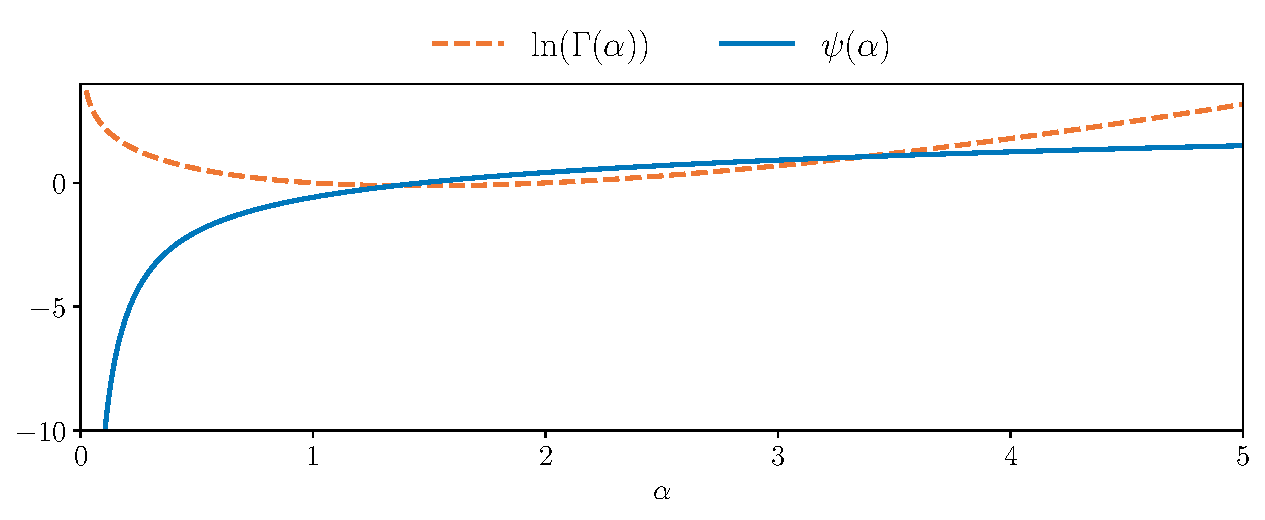
\includegraphics[width=1.0\linewidth]{chapter_5/figures/digamma.pdf}
    \caption[Plot of the Digamma Function and its Derivative]{Plot of the Digamma function $\psi(\cdot)$ in the plain blue curve and its derivative $\ln(\Gamma(\cdot))$ (\ie, the logarithm of the Gamma function $\Gamma(\cdot)$) in the dotted orange curve.}
    \label{chap:mv-sto:fig:digamma}
\end{figure}

Note, while the bound shown in this theorem is based on \citeauthor{Seeger2002}’s form, our contribution does not restrict the choice of generalization bounds.
Indeed, one can derive other versions of the bound based on \citeauthor{McAllester1998} or \citeauthor{Catoni2007}'s approach. 
As we will see in Section~\ref{chap:mv-sto:sec:algo}, 
we make use of \Cref{chap:mv-sto:theorem:bound} to derive a new learning algorithm for the stochastic majority vote. 

As we have seen previously (notably in \Cref{chap:pac-bayes:sec:pac-bayes}), the higher the KL divergence $\KL\LP\hyperQ\|\hyperP\RP$, the more different the two distributions $\hyperQ$ and $\hyperP$ are.
In this context, an increase of the Dirichlet parameters $\paramDir$ can result in the increase of the KL divergence and a concentration of the Dirichlet distribution (see \Cref{chap:mv-sto:fig:dirichlet}).
Indeed, when the parameters $\paramDir$ increase, the stochastic majority vote risks tends to the risk of the majority vote with weight $\frac{\sparamDir_i}{\|\paramDir\|_{1}}$ for the voter $i$.
However, at the same time, the parameters increasing, favour a large KL divergence: the bound is a trade-off between the risk's concentration and the KL divergence.
For now, \Cref{chap:mv-sto:theorem:bound} has a major drawback: it assumes that the voters are not dependent on the learning sample $\S$.
Hence, to overcome this issue, we derive in \Cref{chap:mv-sto:sec:bound-data} a PAC-Bayesian bound that allows us to have data-dependent voters.

\subsection{A PAC-Bayesian Bound for Data-dependent Voters}
\label{chap:mv-sto:sec:bound-data}

\looseness=-1
Importantly, Theorem~\ref{chap:mv-sto:theorem:bound} holds when the hyper-prior $\hyperP$ and the set of voters $\H$ are defined \apriori, \ie, they are independent from the data $\S\sim\D^{\m}$.
However, it is known that considering a data-dependent prior can lead to tighter PAC-Bayes bounds~\citep{ParradoHernandezAmbroladzeShaweTaylorSun2012,DziugaiteHsuGharbiehArpinoRoy2021}.
Following recent works on PAC-Bayesian bounds with data-dependent priors~\citep{ThiemannIgelWintenbergerSeldin2017,MhammediGrunwaldGuedj2019}, we derive a generalization bound that allows us to learn the voters from an additional set.
More precisely, we consider two independent training sets $\S_1$ and $\S_2$ and we learn a set of voters on each training set (determining the set of voters $\H_1$ and $\H_2$).
We refer to the hyper-prior distribution over $\H_1$ \resp over $\H_2$ as $\hyperP_1$ \resp $\hyperP_2$.
In the same way, we can then define a hyper-posterior distribution per voters' set: $\hyperQ_1$ and $\hyperQ_2$.
The following theorem shows that we can bound the risk of two combined stochastic majority votes, as long as their empirical risks are evaluated on the data split that was not used for learning their respective voters.

\begin{restatable}[PAC-Bayesian bound with data-dependent voters]{theorem}{theorembounddata}\label{chap:mv-sto:theorem:bound-data}
Let $\hyperP_1$ and $\hyperQ_1$ be the hyper-prior and hyper-posterior distributions on $\H_1$ defined with $\S_1$, and $\hyperP_2$ and $\hyperQ_2$ the prior and posterior distributions on $\H_2$ defined with $\S_2$.
For any $\lambda \in [0, 1]$ and $\delta \in (0,1]$ with probability at least $1{-}\delta$ over samples $\S_1\sim\D^{\m_1}$ and $\S_2\sim\D^{\m_2}$, 
we have
\begin{align*}
    &\lambda\EE_{\Q\sim\hyperQ_1}\!\Risk_{\D}(\MVQ) + (1{-}\lambda)\EE_{\Qp\sim\hyperQ_2}\!\Risk_{\D}(\MVQp) \le \EE_{(\x,\y)\sim\D}\LB \lambda s_{\hyperQ_1}(\x,\y){+}(1{-}\lambda)s_{\hyperQ_2}(\x,\y) \RB \le\\ 
    &\klmax\!\LB \EE_{(\x,\y)\sim\dS_1}\!\!\frac{s_{\hyperQ_1}(\x, \y)}{\tfrac{1}{\lambda}}{+}\!\!\EE_{(\x,\y)\sim\dS_2}\!\!\frac{s_{\hyperQ_2}(\x, \y)}{\tfrac{1}{1{-}\lambda}} \;\middle|\; \frac{\KL(\hyperQ_1\|\hyperP_1){+}\ln\tfrac{4\sqrt{\m}}{\delta}}{\frac{\m}{\lambda}}{+}\frac{\KL(\hyperQ_2\|\hyperP_2){+}\ln\tfrac{4\sqrt{\mp}}{\delta}}{\frac{\mp}{1{-}\lambda}}\RB\!.
\end{align*}
\end{restatable}
\begin{noaddcontents}\begin{proof}
Deferred to~\Cref{chap:mv-sto:sec:proof-theorem-bound-data}.
\end{proof}\end{noaddcontents}

Following~\citet{MhammediGrunwaldGuedj2019} we set $\lambda=0.5$ and we applied a 50\%/50\% split in the training data.
In the case when the number of data points is odd, we evaluate the bound with $\m_2=\card(\S_2)-1$ that still gives a correct bound (but simplifies the expression of the bound).
In this case the bound is given in the following corollary.

\begin{restatable}[PAC-Bayesian bound with data-dependent voters]{corollary}{corollarybounddata}\label{chap:mv-sto:corollary:bound-data}
Let $\hyperP_1$ and $\hyperQ_1$ be the hyper-prior and hyper-posterior distributions on $\H_1$, and $\hyperP_2$ and $\hyperQ_2$ the prior and posterior distributions on $\H_2$.
For any $\delta \in (0,1)$ with probability at least $1{-}\delta$ over samples $\S_1\sim\D^{\m_1}$ and $\S_2\sim\D^{\m_2}$, 
we have
\begin{align*}
    &\frac{1}{2}\LB\EE_{\Q\sim\hyperQ_1}\!\Risk_{\D}(\MVQ) +\EE_{\Qp\sim\hyperQ_2}\!\Risk_{\D}(\MVQp)\RB \le \EE_{(\x,\y)\sim\D} \frac{1}{2}\LB s_{\hyperQ_1}(\x,\y){+}s_{\hyperQ_2}(\x,\y) \RB \le\\ 
    &\klmax\!\LB \frac{1}{2}\!\LP\EE_{(\x,\y)\sim\dS_1}\!\!s_{\hyperQ_1}(\x, \y){+}\!\!\EE_{(\x,\y)\sim\dS_2}\!\!s_{\hyperQ_2}(\x, \y)\RP \;\middle|\; \frac{\KL(\hyperQ_1\|\hyperP_1){+}\KL(\hyperQ_2\|\hyperP_2){+}2\ln\tfrac{4\sqrt{\m}}{\delta}}{\m}\RB\!,
\end{align*}
where $\m=2\lfloor\frac{\m_1{+}\m_2}{2}\rfloor$ and $\lfloor\cdot\rfloor$ is the floor function.
\end{restatable}

As for \Cref{chap:mv-sto:theorem:bound}, the true risk of two combined stochastic majority votes is upper-bounded by a PAC-Bayesian bound that depends on two terms.
Indeed, it depends on the empirical risk of the two stochastic majority votes and two KL divergences between the hyper-priors and the hyper-posteriors.
This bound is evaluated in practice (in \Cref{chap:mv-sto:sec:expe}) when considering the data-dependent voters. 

\subsection{Learning Algorithms for the Stochastic Majority Vote}
\label{chap:mv-sto:sec:algo}

\looseness=-1
As in \Cref{chap:mv-robustness,chap:mv}, we derive a self-bounding algorithm~\citep{Freund1998} from \Cref{chap:mv-sto:theorem:bound} and \Cref{chap:mv-sto:corollary:bound-data}.
We based the derivation such an algorithm on the stochastic gradient descent. 
To do so, we consider mini-batches $\batch\subseteq\S$ to optimize the generalization bounds.
More precisely, the considered objective function for \Cref{chap:mv-sto:theorem:bound} is  
\begin{align}
    \StoObjbatch \defeq \klmax\LP \EE_{(\x,\y)\sim\dbatch}s_{\hyperQ}(\x, \y) \;\middle|\; \frac{\KL(\hyperQ\|\hyperP){+}\ln\frac{2\sqrt{m}}{\delta}}{\m}\RP,\label{chap:mv-sto:eq:obj-bound}
\end{align}
which is the upper bound applied on the mini-batch $\batch$.
To optimize such an objective function, we apply \Cref{chap:mv-sto:algo:not-data} in conjunction with \Cref{chap:mv-sto:algo:mc} when we approximate the empirical stochastic risks or \Cref{chap:mv-sto:algo:exact} when we compute the risk exactly; the algorithm is summarized in the following algorithm.

\begin{algorithm}[H]
 \caption{Minimization of \Cref{chap:mv-sto:theorem:bound}'s Bound}
 \begin{algorithmic}
 \State{{\bf Given: } learning sample $\S$, hyper-prior distribution $\hyperP$ on $\H$}
 \State{{\bf Hyperparameters: } number of iterations $\iter$}
 \State{$\hyperQ \leftarrow \hyperP$}
 \For{$\t\leftarrow 1$ to $\iter$}
 \For{{\bf all} mini-batches $\batch\subseteq\S$}
    \State{Compute the empirical stochastic risk $\EE_{(\x,\y)\sim\dbatch}s_{\hyperQ}(\x, \y)$}
    \State{with \Cref{chap:mv-sto:algo:mc} or \Cref{chap:mv-sto:algo:exact}}
    \State{$\hyperQ\leftarrow$ Update $\hyperQ$ with $\StoObjbatch$ by gradient descent}
 \EndFor
 \EndFor
 \State{\Return{$\hyperQ$}}
 \end{algorithmic}
 \label{chap:mv-sto:algo:not-data}
\end{algorithm}

For each iteration we compute the empirical risk on the mini-batch $\batch$.
To do so, the risk is either approximated with \Cref{chap:mv-sto:algo:mc} or computed exactly with \Cref{chap:mv-sto:algo:exact}.
Then, we compute the objective function and update the hyper-posterior $\hyperQ$ with a gradient descent algorithm.
For the data-dependent voters version, similarly as \Cref{chap:mv-sto:corollary:bound-data} which relies on the presence of two learning samples $\S_1$ and $\S_2$, the objective function is defined as
\begin{align}
\MulStoObjbatch \defeq \klmax\Bigg[ \frac{1}{2}\!\Bigg(\EE_{(\x,\y)\sim\dbatch_1}\!\!s_{\hyperQ_1}(\x, \y)&{+}\!\!\EE_{(\x,\y)\sim\dbatch_2}\!\!s_{\hyperQ_2}(\x, \y)\Bigg)\nonumber\\
&\Bigg|\; \frac{\KL(\hyperQ_1\|\hyperP_1){+}\KL(\hyperQ_2\|\hyperP_2){+}2\ln\tfrac{4\sqrt{\m}}{\delta}}{\m}\Bigg].\label{chap:mv-sto:eq:obj-bound-data}
\end{align}

This objective function estimated through a mini-batch $\batch_1$ from $\S_1$ and $\batch_2$ from $\S_2$. 
Similarly as \Cref{chap:mv-sto:eq:obj-bound}, the objective function in \Cref{chap:mv-sto:eq:obj-bound-data} estimates the upper-bound of \Cref{chap:mv-sto:theorem:bound-data}.
The algorithm considered to minimize such a bound is described in \Cref{chap:mv-sto:algo:not-data}.

\begin{algorithm}[H]
 \caption{Minimization of \Cref{chap:mv-sto:corollary:bound-data}'s Bound}
 \begin{algorithmic}
 \State{{\bf Given: } learning samples $\S_1$ and $\S_2$, hyper-priors $\hyperP_1$ on $\H_1$ and $\hyperP_2$ on $\H_2$}
 \State{{\bf Hyperparameters: } number of iterations $\iter$}
 \State{$(\hyperQ_1, \hyperQ_2)  \leftarrow (\hyperP_1, \hyperP_2)$}
 \For{$\t\leftarrow 1$ to $\iter$}
 \For{{\bf all} mini-batches $\batch_1\subseteq\S_1$ and $\batch_2\subseteq\S_2$}
    \State{Compute the empirical stochastic risks $\EE_{(\x,\y)\sim\dbatch_1}s_{\hyperQ_1}(\x, \y)$ and}
    \State{$\EE_{(\x,\y)\sim\dbatch_2}s_{\hyperQ_2}(\x, \y)$ with \Cref{chap:mv-sto:algo:mc} or \Cref{chap:mv-sto:algo:exact}}
    \State{$(\hyperQ_1, \hyperQ_2)\leftarrow$ Update $\hyperQ_1$ and $\hyperQ_2$ with $\MulStoObjbatch$ by gradient descent}
 \EndFor
 \EndFor
 \State{\Return{$(\hyperQ_1, \hyperQ_2)$}}
 \end{algorithmic}
 \label{chap:mv-sto:algo:data}
\end{algorithm}

For each iteration of the algorithm, the two stochastic risks are computed with \Cref{chap:mv-sto:algo:mc} or \Cref{chap:mv-sto:algo:exact}.
Then, thanks to these two values, we can compute the objective function $\MulStoObjbatch$ (\Cref{chap:mv-sto:eq:obj-bound-data}).
Finally, the hyper-posteriors $\hyperQ_1$ and $\hyperQ_2$ are updated through a gradient descent step.

\paragraph{Computing the derivatives.}
When the risk is computed from \Cref{chap:mv-sto:algo:mc}, the sum is differentiable.
However, since the risk is obtained by a Monte Carlo sampling, we use the implicit reparameterization trick~\citep{FigurnovMohamedMnih2018, JankowiakObermeyer2018} to obtain the derivatives; it is directly implemented in the automatic differentiation framework such as \pytorch~\citep{Paszke2019}.
Moreover, when the closed form solution (derived in \Cref{chap:mv-sto:corollary:risk}) risk is computed through \Cref{chap:mv-sto:algo:exact}, the risk depends on the function $I_{0.5}()$ which is differentiable as well~\citep[see][]{BoikRobinsonCox1999}.\\

In the following section, we evaluate \Cref{chap:mv-sto:algo:not-data,chap:mv-sto:algo:data} and compared them with the algorithms of \Cref{chap:mv}.

\section{Experiments}
\label{chap:mv-sto:sec:expe}

In this section, we compare the generalization bounds and the test risks obtained with our algorithms and the ones in \Cref{chap:mv}.
We show that our algorithms allow us to derive generalization bounds that are tight and non-vacuous (\ie, smaller than $1$) with decision stumps and decision trees.\\

We consider as baselines the following PAC-Bayesian self-bounding algorithms: 
\begin{enumerate}[label={\it (\roman*)}]
    \item The algorithm \algogermain that minimizes the PAC-Bayesian of \citet[PAC-Bound 0]{GermainLacasseLavioletteMarchandRoy2015} on $2r_{\D}(\Q)$ (\Cref{chap:pac-bayes:theorem:2gibbs}),
    \item The algorithm \algomasegosa of \citet{MasegosaLorenzenIgelSeldin2020} minimizing a PAC-Bayesian bound on $4e_{\D}(\Q)$ (\Cref{chap:pac-bayes:theorem:4joint}),
    \item \Cref{chap:mv:algo:seeger} minimizing the PAC-Bayesian C-Bound based on \citeauthor{Seeger2002}'s approach (\Cref{chap:mv:theorem:cbound-seeger}),
    \item \algolacasse~\citep{LacasseLavioletteMarchandTurgeonBoutin2010} minimizes \Cref{chap:mv-sto:eq:lacasse} for a majority vote that samples $N$ voters from $\Q$.
\end{enumerate}

The parameters of the baseline are the same as in \Cref{chap:mv:sec:expe}.
For \algolacasse the number of voters drawn is set to $N{=}100$.
As in \Cref{chap:mv} the generalization bounds are evaluated with $\delta=0.05$ and the sigmoid's slope parameter $c$ is set to $100$ for \Cref{chap:mv-sto:algo:exact}.
Moreover, the values are averaged over $10$ runs.

\subsection{Comparison Between the Computations of the Risk}
\label{chap:mv-sto:sec:exact-mc}

For this set of experiments, we optimize \Cref{chap:mv-sto:theorem:bound} with \Cref{chap:mv-sto:algo:not-data}, for $\iter=2,000$ iterations with COCOB-Backprop optimizer~\citep{OrabonaTommasi2017}.
We study the performance of our method on the binary classification moons dataset, with $2$ features, $2$ classes and $\Ncal(0, 0.05)$ Gaussian noise, for which we draw $\m$ points for training, and $\card(\T)=2,000$ points for testing.\\

\Cref{chap:mv-sto:fig:moons-voter} reports a comparison of \Cref{chap:mv-sto:algo:mc,chap:mv-sto:algo:exact} in terms of test risk $\EE_{\Q\sim\hyperQ}\Risk_{\dT}(\MVQ)$, PAC-Bayesian generalization bound and training time when the number of decision stumps increases (with $\m=2,000$).
We observe that the test risks and bound values can degrade for higher values of decision stumps for all methods.
This is due to the KL divergence increasing with the number of voters $\card(\H)$, as highlighted in \Cref{ap:mv-sto:sec:result}, becoming a too strong regularization during training and making the bound looser. 
Moreover, when the number of decision stumps increases, \Cref{chap:mv-sto:algo:exact} can be quicker than \Cref{chap:mv-sto:algo:mc} especially when the Monte Carlo draws $\K$ is high compared to $\m$. 

We report in \Cref{chap:mv-sto:fig:moons-size} the evolution of the test risk $\EE_{\Q\sim\hyperQ}\Risk_{\dT}(\MVQ)$, PAC-Bayesian bounds and training time when $\m$ increases.
When $\m$ is large enough, \Cref{chap:mv-sto:algo:mc} achieves comparable test risk and bound values compared to \Cref{chap:mv-sto:algo:exact} even for $\K=1$.
Increasing the number of Monte Carlo draws $\K$ unsurprisingly allows to recover \Cref{chap:mv-sto:algo:exact}'s performance, and at lower computational cost for reasonable values of $\m$ and $\K$.

\begin{figure}
    \centering
    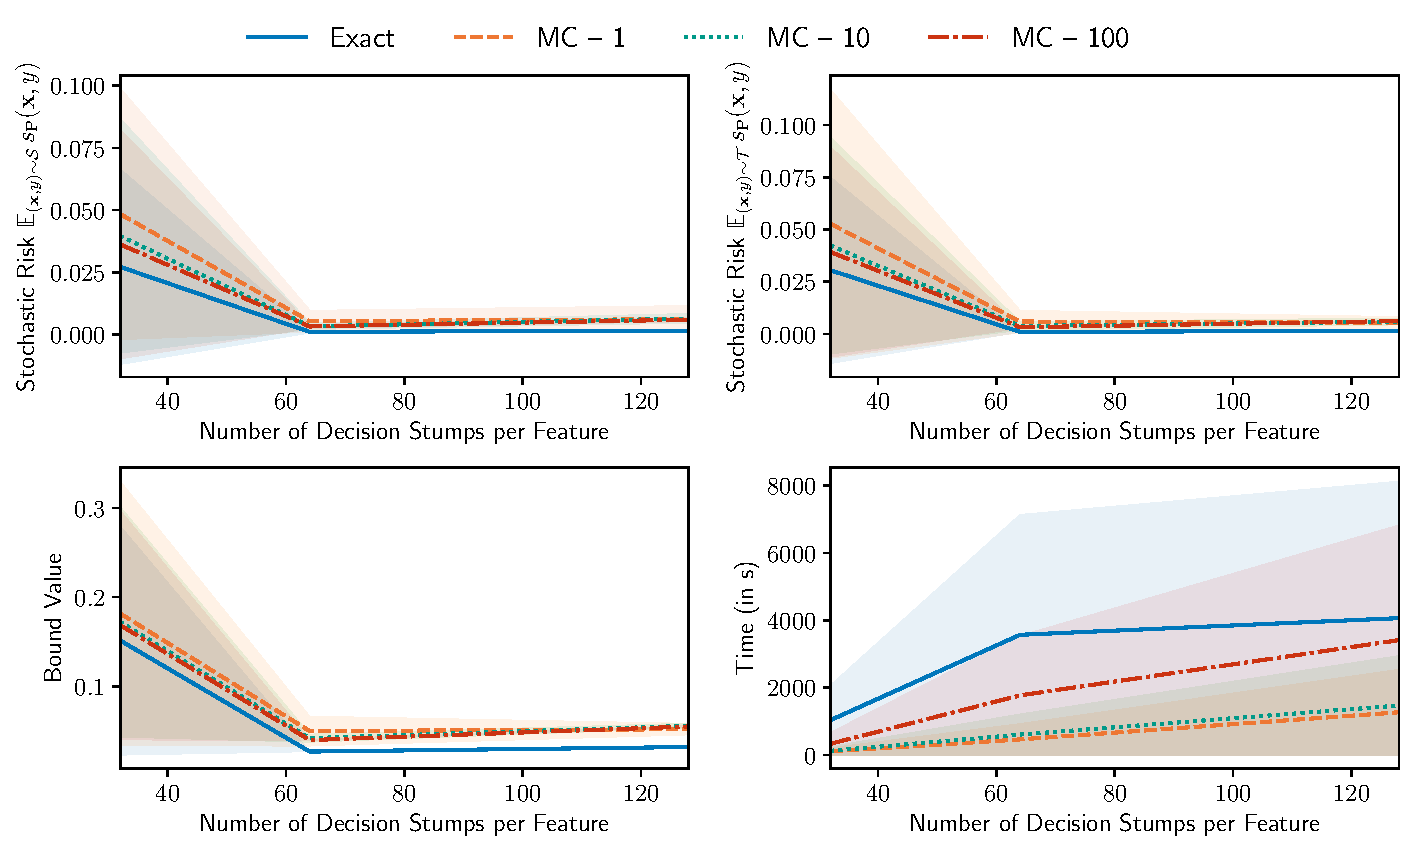
\includegraphics[width=1.0\linewidth]{chapter_5/figures/moons_voter.pdf}
    \caption[Plot of the Performance of \Cref{chap:mv-sto:algo:mc,chap:mv-sto:algo:exact} on Moons (1/2)]{Plot of the average performance on 10 runs of \Cref{chap:mv-sto:algo:mc} (with $\K\in\{1, 10, 100\}$) and \Cref{chap:mv-sto:algo:exact} as a function of the number of decision stumps per feature with learning sample size $\m=2000$.}
    \label{chap:mv-sto:fig:moons-voter}
\end{figure}

\begin{figure}
    \centering
    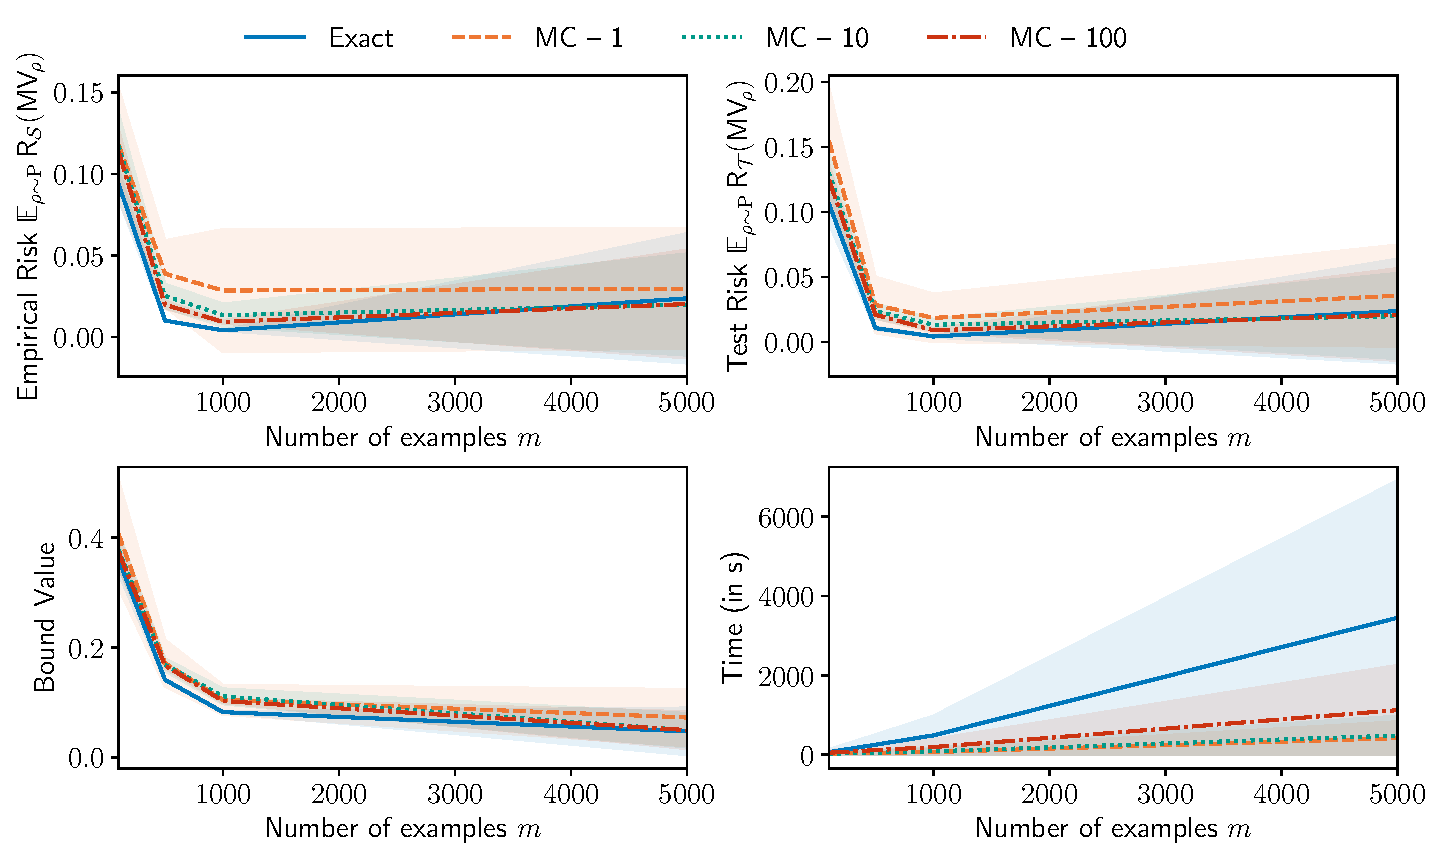
\includegraphics[width=1.0\linewidth]{chapter_5/figures/moons_size.pdf}
    \caption[Plot of the Performance of \Cref{chap:mv-sto:algo:mc,chap:mv-sto:algo:exact} on Moons (2/2)]{Plot of the average performance on 10 runs of \Cref{chap:mv-sto:algo:mc} (with $\K\in\{1, 10, 100\}$) and \Cref{chap:mv-sto:algo:exact} as a function of the learning sample size $\m$ with 32 decision stump per feature.}
    \label{chap:mv-sto:fig:moons-size}
\end{figure}

\subsection{Performance of \Cref{chap:mv-sto:algo:data,chap:mv-sto:algo:not-data}}

We now compare \Cref{chap:mv-sto:algo:not-data,chap:mv-sto:algo:data} on different datasets namely \mbox{FashionMNIST}~\citep{XiaoRasulVollgraf2017}, MNIST~\citep{LeCunCortesBurges1998} and datasets coming from the UCI repository~\citep{DuaGraff2017}; the processing of the dataset is the same as in \Cref{chap:mv:sec:expe}.
More precisely, the same number of examples is kept in the test or the train set as in the original split.
When no original split was proposed, we use 50\% of data in the training set $\S$ and 50\% in the test set (except for Sensorless where we have 15\% in the test set).
When making use of {\it data-independent voters}, we chose decision stumps as voters;
When making use of {\it data-dependent voters}, we build decision trees as set of voters without bounding their maximal depth (unless stated otherwise).
The voters are exactly the same as in \Cref{chap:mv}.

\begin{figure}
    \centering
    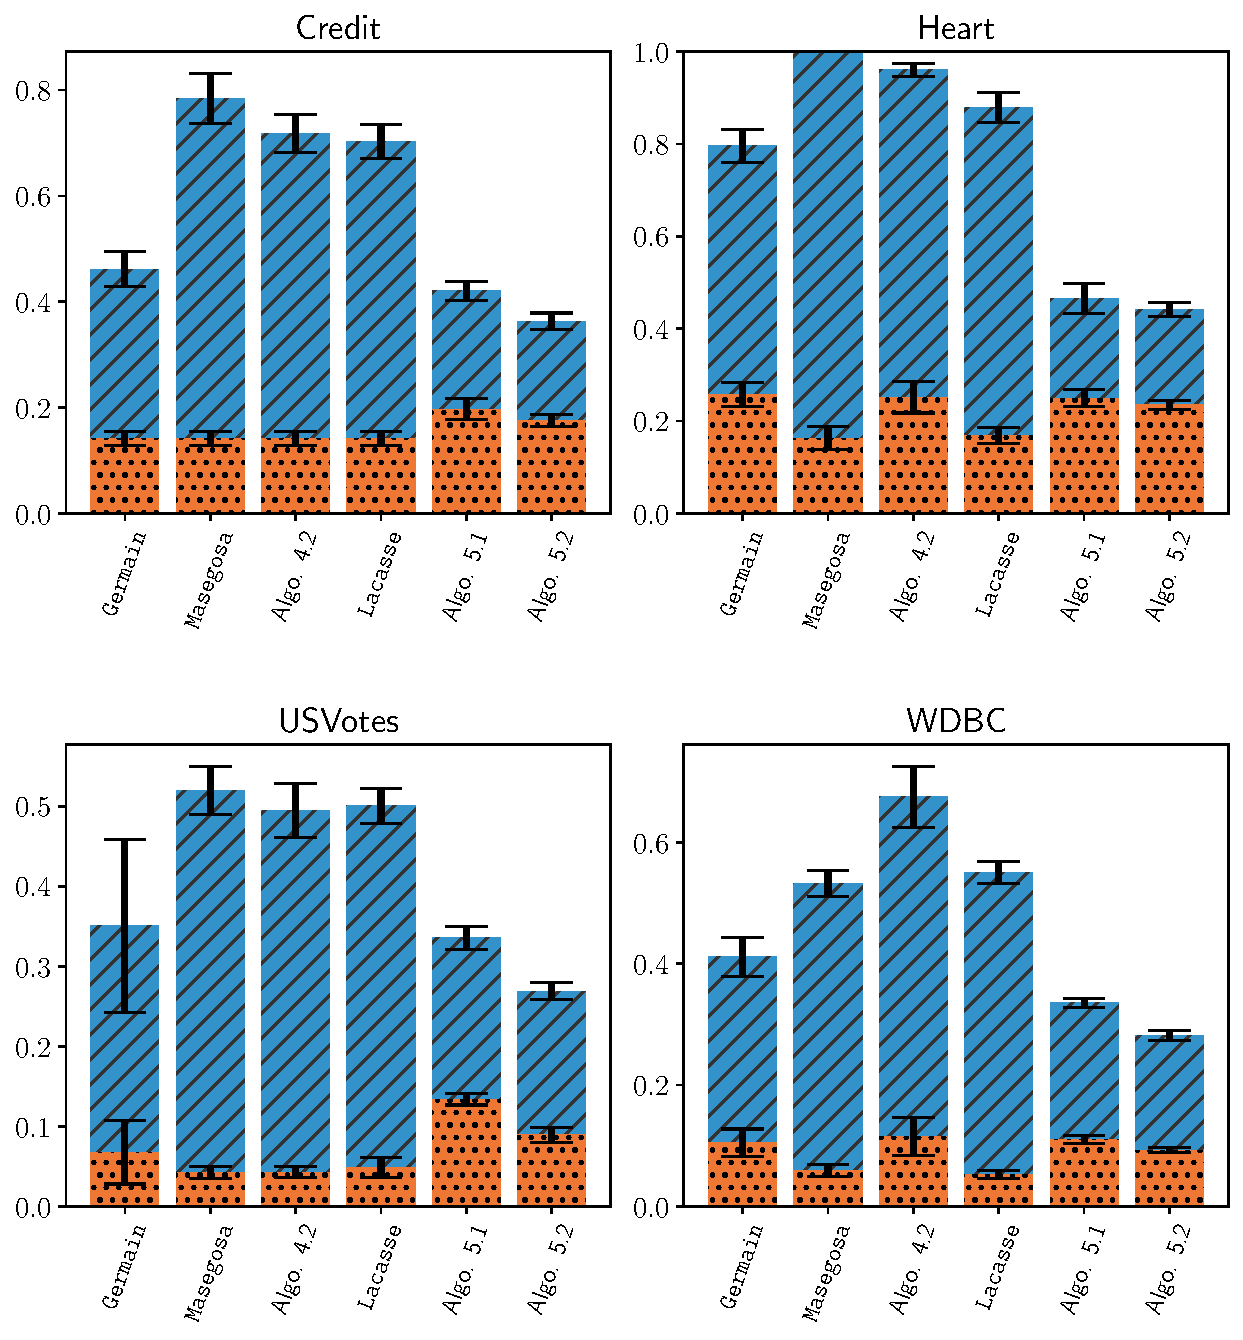
\includegraphics[width=1.0\linewidth]{chapter_5/figures/stump_binary_1.pdf}
    \caption[Comparison of the Risks and the Bound Values (1/4)]{
    Comparison in terms of test risks, stochastic test risks and bound values. 
    We report in the dotted orange error bars, the means and standard deviations of the test risks and stochastic risks.
    Moreover, the hatched blue error bars represent the mean and the standard deviations of the PAC-Bayesian bounds.
    The values are average over 10 different runs.
    }
    \label{chap:mv-sto:fig:stump-binary-1}
\end{figure}

\begin{figure}
    \centering
    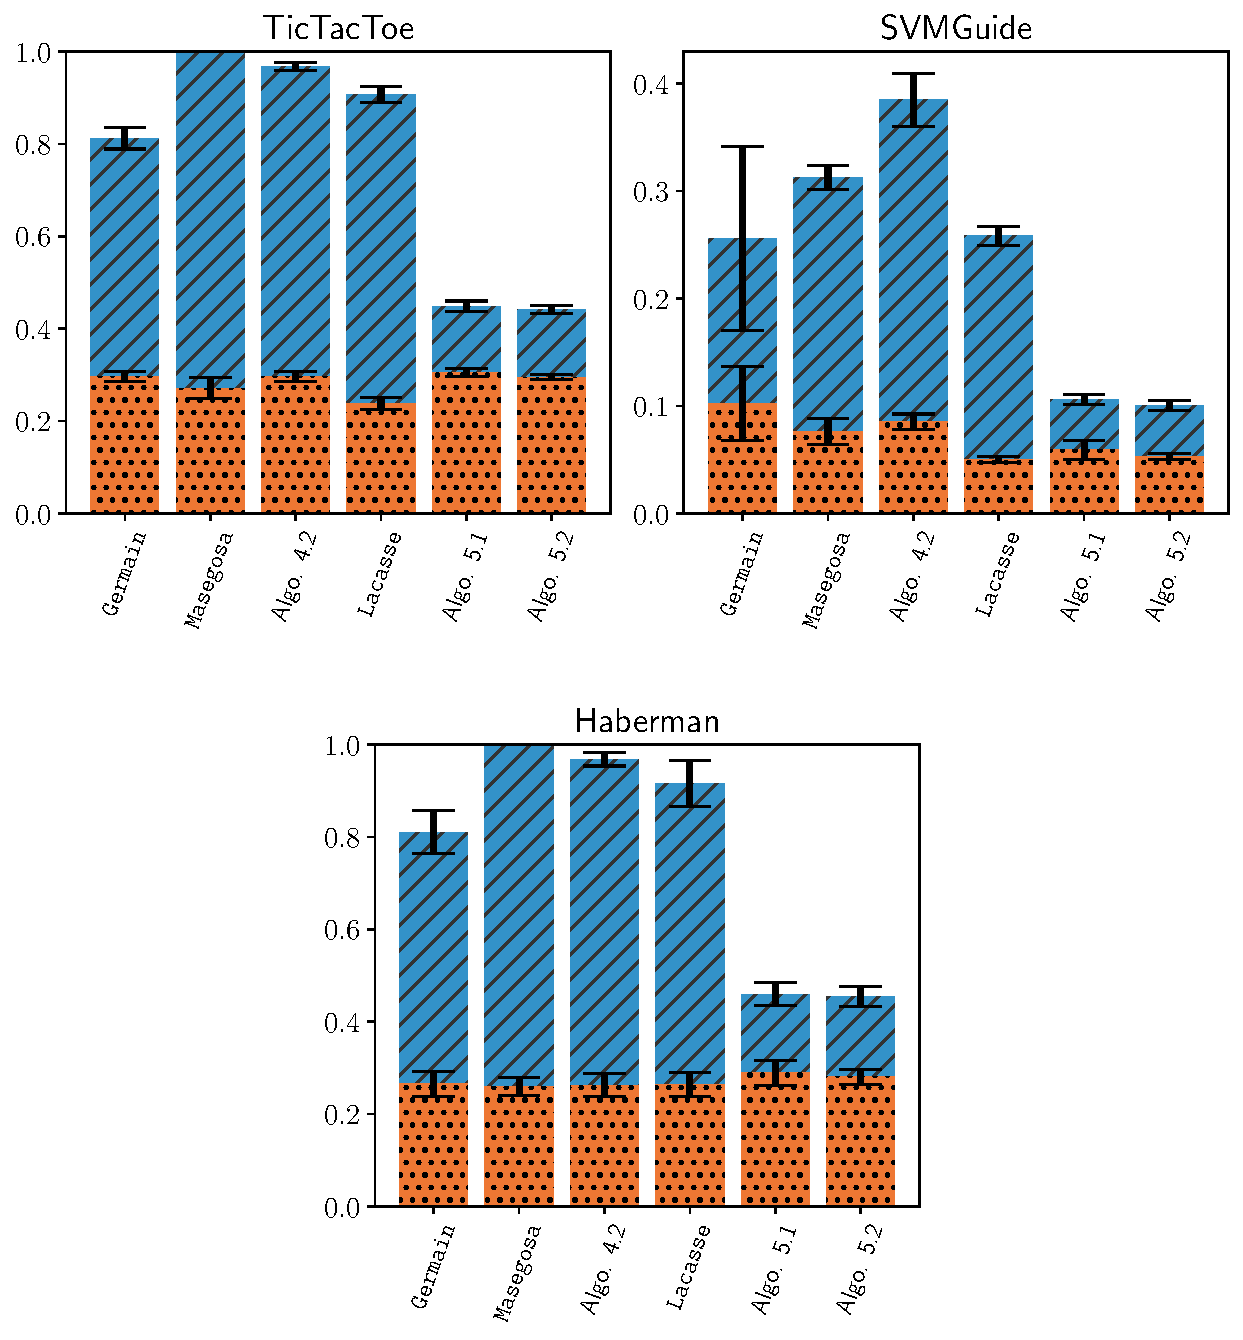
\includegraphics[width=1.0\linewidth]{chapter_5/figures/stump_binary_2.pdf}
    \caption[Comparison of the Risks and the Bound Values (2/4)]{
    Comparison in terms of test risks, stochastic test risks and bound values. 
    We report in the dotted orange error bars, the means and standard deviations of the test risks and stochastic risks.
    Moreover, the hatched blue error bars represent the mean and the standard deviations of the PAC-Bayesian bounds.
    The values are average over 10 different runs.
    }
    \label{chap:mv-sto:fig:stump-binary-2}
\end{figure}

\begin{figure}
    \centering
    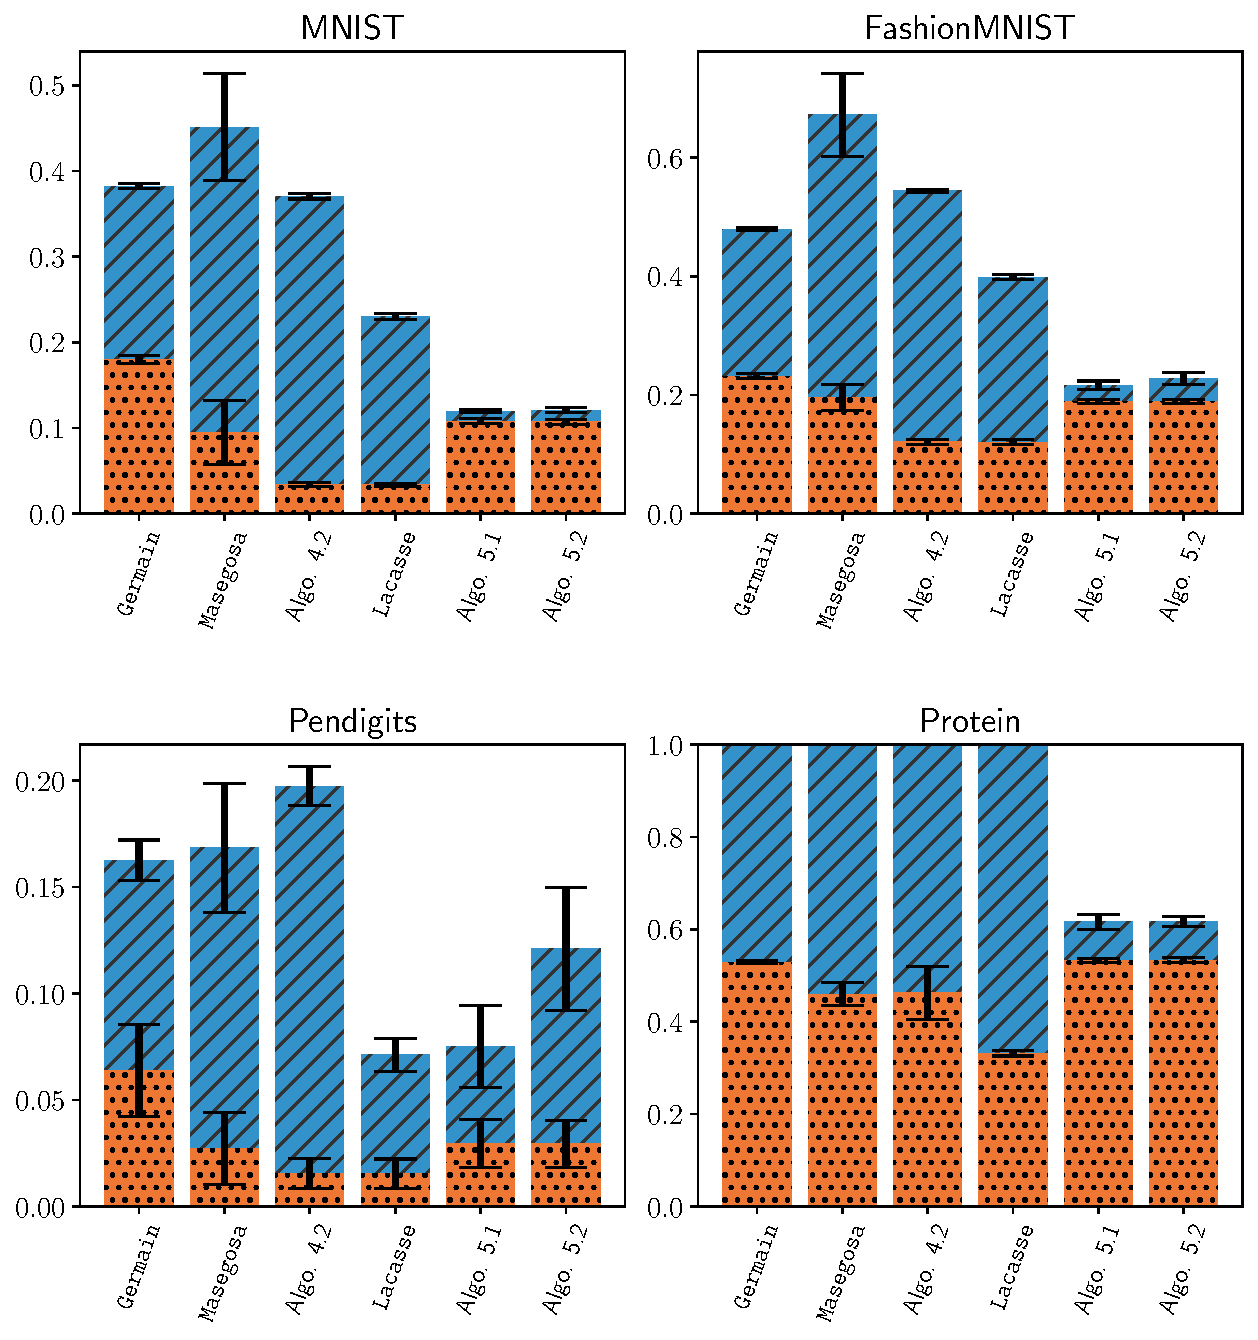
\includegraphics[width=1.0\linewidth]{chapter_5/figures/tree_multi_1.pdf}
    \caption[Comparison of the Risks and the Bound Values (3/4)]{
    Comparison in terms of test risks, stochastic test risks and bound values. 
    We report in the dotted orange error bars, the means and standard deviations of the test risks and stochastic risks.
    Moreover, the hatched blue error bars represent the mean and the standard deviations of the PAC-Bayesian bounds.
    The values are average over 10 different runs.
    }
    \label{chap:mv-sto:fig:stump-multi-1}
\end{figure}

\begin{figure}
    \centering
    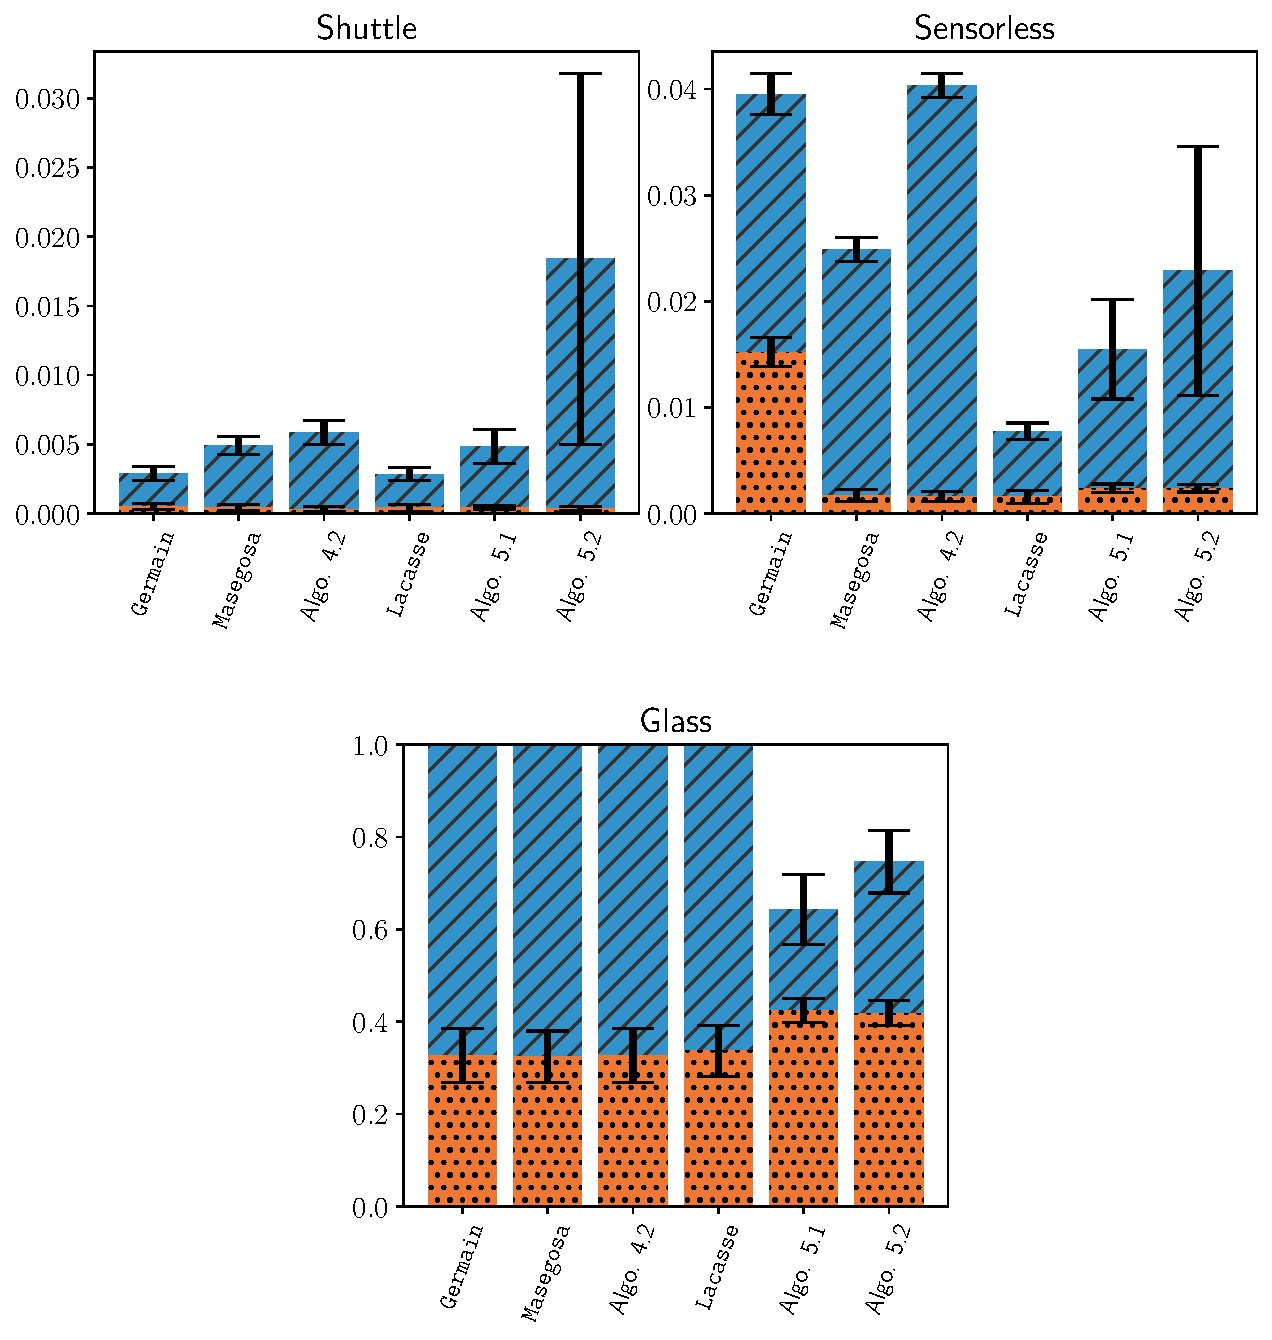
\includegraphics[width=1.0\linewidth]{chapter_5/figures/tree_multi_2.pdf}
    \caption[Comparison of the Risks and the Bound Values (4/4)]{
    Comparison in terms of test risks, stochastic test risks and bound values. 
    We report in the dotted orange error bars, the means and standard deviations of the test risks and stochastic risks.
    Moreover, the hatched blue error bars represent the mean and the standard deviations of the PAC-Bayesian bounds.
    The values are average over 10 different runs.
    }
    \label{chap:mv-sto:fig:stump-multi-2}
\end{figure}

We train the stochastic majority vote models by Stochastic Gradient Descent (SGD) using COCOB-Backprop~\citep{OrabonaTommasi2017} with batch size equal to $64$.
We fix the number of epochs to $20$ and for \Cref{chap:mv-sto:algo:mc} we fix $\K=10$ to increase randomness.

We report the stochastic test risks $\EE_{(\x,\y)\sim\dT}s_{\hyperQ}(\x, \y)$ for our algorithms, the test risk $\Risk_{\dT}(\MVQ)$ for the others and the generalization bounds in \Cref{chap:mv-sto:fig:stump-binary-1,chap:mv-sto:fig:stump-binary-2,chap:mv-sto:fig:stump-multi-1,chap:mv-sto:fig:stump-multi-2} (additional results are reported in \Cref{ap:mv-sto:sec:result}).
More precisely, we compare the different self-bounding algorithms with \Cref{chap:mv-sto:algo:not-data} on binary datasets in \Cref{chap:mv-sto:fig:stump-binary-1,chap:mv-sto:fig:stump-binary-2}, and on multi-class datasets with data-dependent voters and \Cref{chap:mv-sto:algo:data} in \Cref{chap:mv-sto:fig:stump-multi-1,chap:mv-sto:fig:stump-multi-2}.
First, we remark that \Cref{chap:mv-sto:algo:not-data,chap:mv-sto:algo:data} have similar performance in terms of stochastic test risks and bound values. 
Moreover, note that we notice that the bounds obtained from \Cref{chap:mv-sto:algo:not-data,chap:mv-sto:algo:data} are consistently non vacuous and tighter than those obtained with the other algorithms.
While the risks between the methods are not comparable we remark that the stochastic test risk $\EE_{(\x,\y)\sim\dT}s_{\hyperQ}(\x, \y)$ has similar values than the test risks $\Risk_{\dT}(\MVQ)$.
It means that our algorithms obtain similar test risk $\Risk_{\dT}(\MVQ)$ in expectation (where $\Q\sim\hyperQ$).
We believe that it is due to the fact that the stochastic risks depend on the $\frac{1}{2}$-margin of \citet{LavioletteMorvantRalaivolaRoy2017}.
Indeed, even if our learning algorithms optimizes the 01-loss, it does not fully distinguish examples that are classified correctly or not.

\section{Conclusion and Summary}

In this chapter, we have studied a new type of majority vote: the {\it stochastic majority vote}.
For each input $\x\in\X$, it samples a majority vote $\MVQ$ from a probability distribution called hyper-posterior $\hyperQ$ and output $\MVQ(\x)$.
When the hyper-posterior is a Dirichlet distribution, the stochastic risk can be either approximated or computed exactly.
This allows us to derive a self-bounding algorithm for the stochastic majority vote.
The experiments show that our learning algorithm provides a tight PAC-Bayesian generalization bound along with a small empirical risk.\\

One of the perspectives of this work is to consider the risk of the stochastic majority vote by doing without the $\frac{1}{2}$-margin of \citet{LavioletteMorvantRalaivolaRoy2017}.
However, we may not find the closed-form solution of the stochastic majority vote's risk, in this context.
In other words, the risk might be only approximated by Monte Carlo sampling.
To avoid such a drawback we can make use of a different type of bounds: the {\it disintegrated} PAC-Bayesian bounds.
Indeed, in \Cref{part:contrib-disintegrated}, we study the {\it disintegrated} bounds in more details.
As recalled in \Cref{chap:pac-bayes}, these bounds have been introduced by \citet{Catoni2007,BlanchardFleuret2007} and have been rediscovered lately by \citet{RivasplataKuzborskijSzepesvariShaweTaylor2020}.
They allow us to derive a bound for a {\it single} voter or hypothesis from the hypothesis set $\H$.  
\Cref{chap:dis-pra} introduces new {\it disintegrated} bounds based on the \textsc{Rényi} divergence (that can be used for the stochastic majority vote) and \Cref{chap:dis-mu} presents generalization bounds that are not restrained to the KL divergence or the \textsc{Rényi} one but can depend on a complexity term defined by the users.